\section{Local smoothing for the wave equation}
\subsection{Decoupling for the truncated cone}
Solutions of the wave equation on $\R^{d}$ have Fourier support on a cone.
For this reason a decoupling theorem for functions with Fourier support near the truncated cone $\calC := \Set{(\xi,\abs{\xi}) \given \xi\in\R^{d}, 1 \leq \abs{\xi} \leq 2}$ will be useful.
\begin{theorem}[{\cite[Section 8]{MR3374964}}]
\label{thm:dec-cone}
Let $d\geq 2$, $2 \leq p \leq \infty$, let $\Theta$ be a boundedly overlapping collection of slabs of size $1 \times \delta \times \dotsm \times \delta \times \delta^{2}$ adapted to $\calC$ as in the picture.
\begin{center}
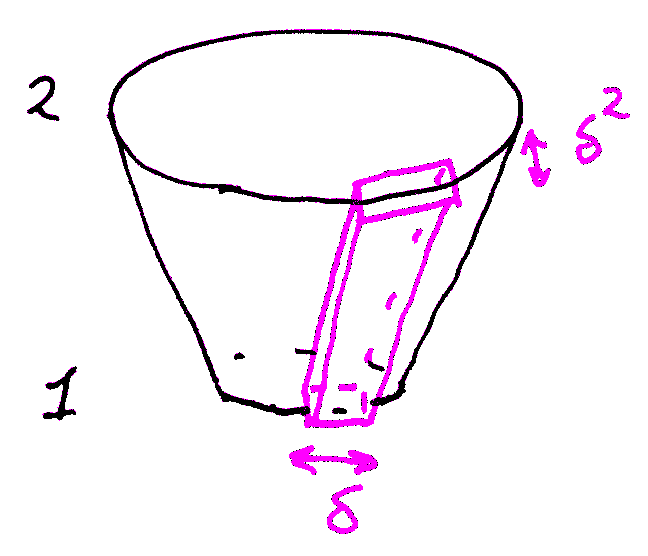
\includegraphics[height=3cm]{cone-slabs.png}
\end{center}
Then for any collection of functions $f_{\theta}$, $\theta\in\Theta$, with $\supp \widehat{f_{\theta}} \subset \theta$ and $\epsilon>0$ we have
\begin{equation}
\label{eq:dec-cone}
\norm[\big]{\sum_{\theta\in\Theta} f_{\theta}}_{p}
\lesssim_{\epsilon} \delta^{-\epsilon-\eta_{p}} \ell^{2}_{\theta\in\Theta} \norm{f_{\theta}}_{p},
\end{equation}
where
\[
\eta_{p} =
\begin{cases}
0, & 2 \leq p \leq 2(d+1)/(d-1),\\
(d-1)/2-(d+1)/p, & 2(d+1)/(d-1) < p \leq \infty.
\end{cases}
\]
\end{theorem}
\begin{proof}
By interpolation, which works similarly to the case of the paraboloid, it suffices to consider the critical exponent $p=2(d+1)/(d-1)$.
Alternatively one could treat all exponents directly.

The main idea is that thin sectors of the cone project to something very close to parabolas along the flat direction of the cone.
Hence we should be able to apply the decoupling theorem for the parabola in dimension $d-1$ fiberwise.
However, the projections are not sufficiently close to the parabola to apply decoupling at scale $\delta$ right away.
Instead we have to set up an induction on scales argument.

Let $M$ be a  positive integer.
For $1\leq m \leq M$ let $\Theta_{m}$ be a boundedly overlapping covering of the thinned cone
\[
\calC' := \Set{(\xi,\abs{\xi}) \given \xi\in\R^{d}, \abs{\xi_{1}-1} \leq \delta^{2/M}, \abs{\xi_{2}} \leq \delta^{1/M}, \dotsc, \abs{\xi_{d}} \leq \delta^{1/M}}
\]
by adapted slabs of size $\sim \delta^{2/M} \times \delta^{m/M} \times \dotsm \times \delta^{m/M} \times \delta^{2m/M}$.
Partition
\[
\Theta_{m+1} = \cup_{\theta \in \Theta_{m}} \Theta_{m+1}(\theta)
\]
in such a way that for $\theta' \in \Theta_{m+1}(\theta)$ we have $\theta' \cap \theta \neq \emptyset$.
Let $f_{\theta'}$, $\theta' \in \Theta_{M}$ be a collection of functions with $\supp \widehat{f_{\theta'}} \subset \theta'$ and define
\[
f_{\theta} := \sum_{\theta' \in \Theta_{m+1}(\theta)} f_{\theta'}
\]
for $m=M-1,\dotsc,1$ and $\theta\in\Theta_{m}$.
We claim that for each $1\leq m < M$ and each $\theta \in \Theta_{m}$ we have
\begin{equation}
\label{eq:dec-cone-inductive-claim}
\norm[\big]{ f_{\theta} }_{p}
\lesssim_{\epsilon,M} \delta^{-\epsilon}
\ell^{2}_{\theta' \in \Theta_{m+1}(\theta)} \norm{ f_{\theta'} }_{p}.
\end{equation}
\begin{center}
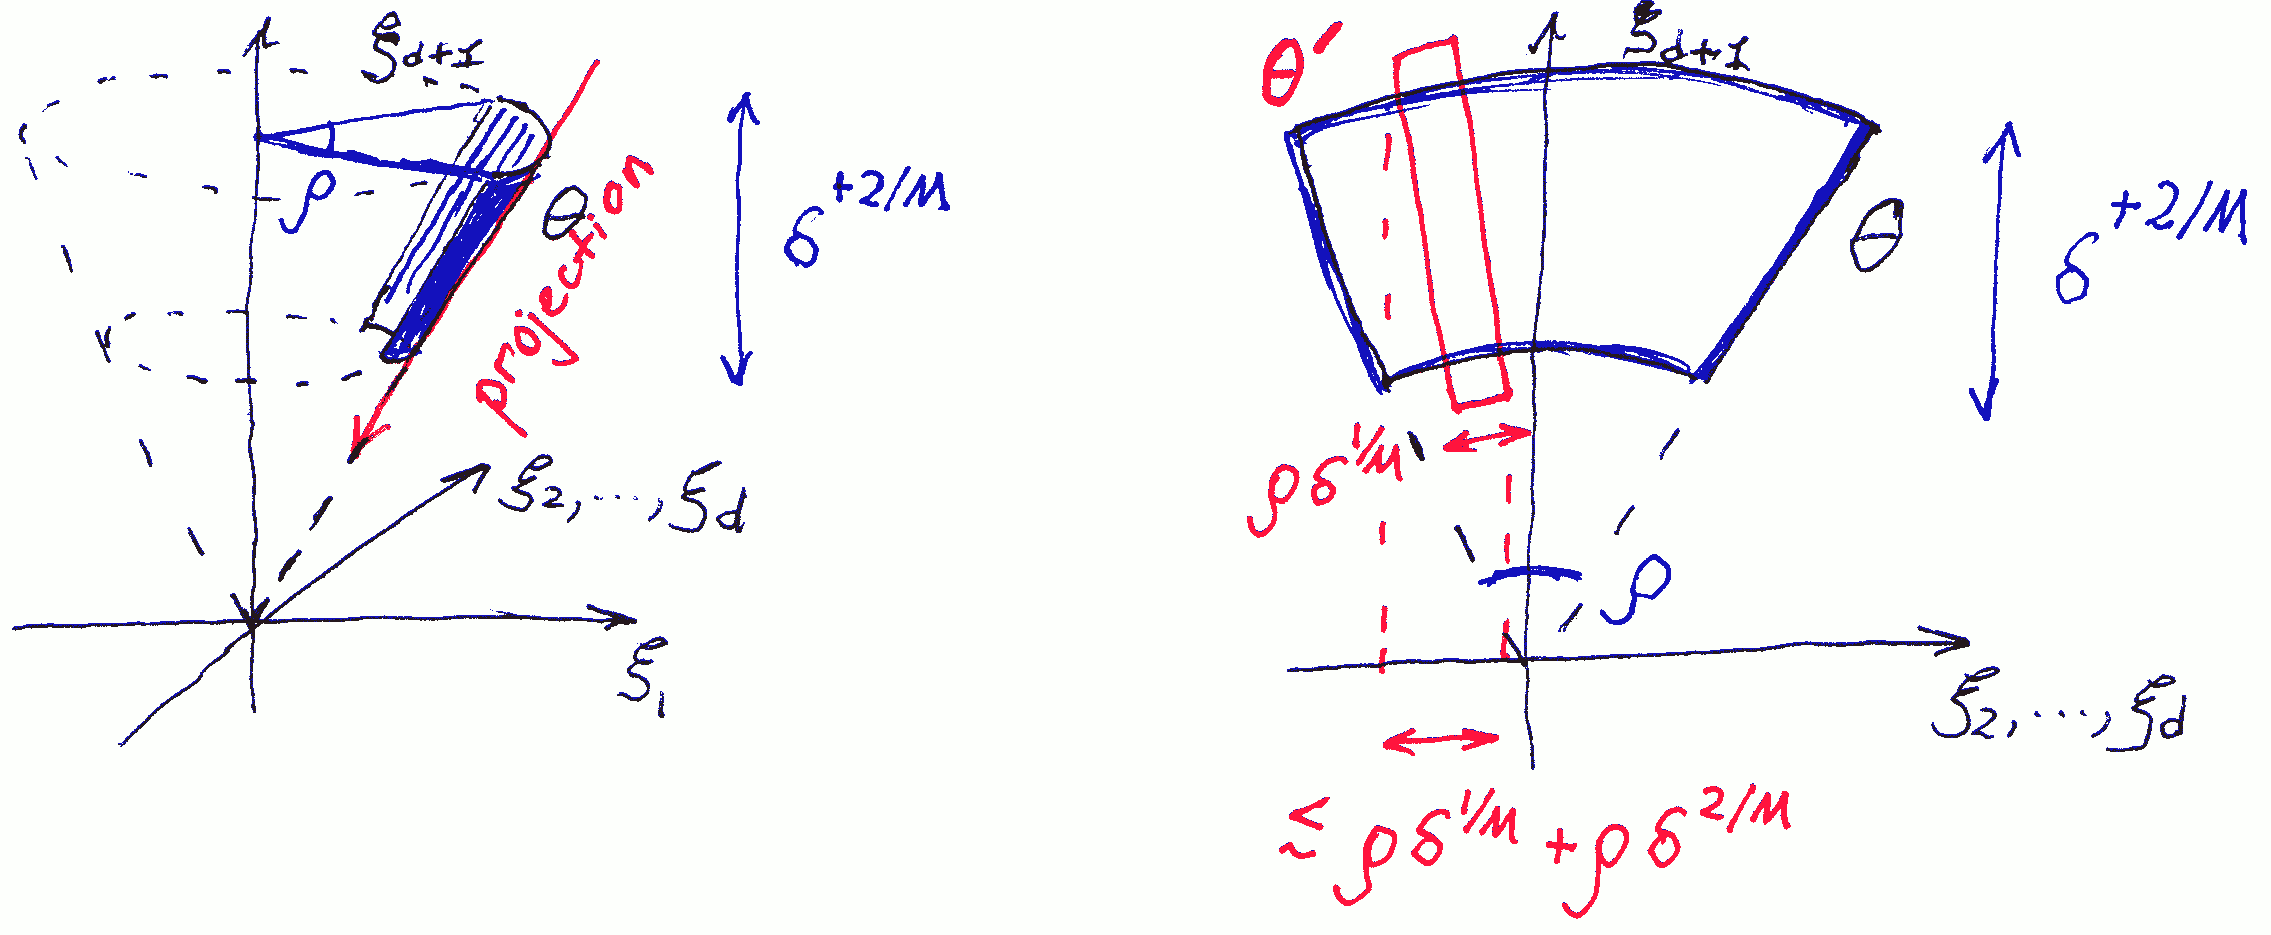
\includegraphics[width=\textwidth]{fig-cone.png}
\end{center}
Iterating the claim \eqref{eq:dec-cone-inductive-claim} we obtain
\[
\norm[\big]{ \sum_{\theta' \in \Theta_{M}} f_{\theta'} }_{p}
\leq
\sum_{\theta \in \Theta_{1}} \norm{f_{\theta}}_{p}
\lesssim
\delta^{-\frac{d-1}{2M}} \ell^{2}_{\theta \in \Theta_{1}} \norm{f_{\theta}}_{p}
\lesssim_{\epsilon,M} \delta^{-\frac{d-1}{2M}-\epsilon}
\ell^{2}_{\theta' \in \Theta_{M}} \norm{ f_{\theta'} }_{p}.
\]
Since we can partition the cone $\calC$ in $O(\delta^{-2/M})$ dilates of the cone $\calC'$ and partition functions $f_{\theta}$ accordingly, the conclusion \eqref{eq:dec-cone} follows with $\epsilon$ replaced by $C/M+\epsilon$.
Since $M$ was arbitrary we obtain \eqref{eq:dec-cone}.

It remains to show the claim \eqref{eq:dec-cone-inductive-claim}.
By rotation invariance we may assume that $\theta$ is adapted to the cone segment
\[
\calC_{\rho} := \Set{(\xi,\abs{\xi}) \given \xi\in\R^{d}, \abs{\xi_{1}-1} \leq \delta^{2/M}, \abs{\xi_{2}}\leq \rho, \dotsc, \abs{\xi_{d}}\leq \rho}
\]
with $\rho = \delta^{m/M}$.
Under the projection map
\[
(\xi_{1},\dotsc,\xi_{d},\xi_{d+1}) \mapsto (\xi_{2},\dotsc,\xi_{d},\xi_{d+1}-\xi_{1})
\]
the parametrization of the cone $\calC_{\rho}$ is mapped to
\[
(\xi_{2},\dotsc,\xi_{d},\sqrt{\xi_{1}^{2}+\dotsb+\xi_{d}^{2}}-\xi_{1}).
\]
Now notice that
\begin{multline*}
\abs[\Big]{\sqrt{\xi_{1}^{2}+\dotsb+\xi_{d}^{2}}-\xi_{1}-\frac{\xi_{2}^{2}+\dotsb+\xi_{d}^{2}}{2}}
=
\abs[\Big]{\frac{\sqrt{\xi_{1}^{2}+\dotsb+\xi_{d}^{2}}^{2}-\xi_{1}^{2}}{\sqrt{\xi_{1}^{2}+\dotsb+\xi_{d}^{2}}+\xi_{1}}-\frac{\xi_{2}^{2}+\dotsb+\xi_{d}^{2}}{2}}\\
\lesssim
\rho^{2}(\sqrt{\xi_{1}^{2}+\dotsb+\xi_{d}^{2}}+\xi_{1}-2)
\lesssim
\rho^{2}\abs{\xi_{1}-1} + \rho^{4}
\lesssim
\rho^{2}\delta^{2/M},
\end{multline*}
so that an $O(\delta^{2})$-neighborhood of $\calC_{\rho}$, and hence $\theta$, is projected to an $O(\rho^{2}\delta^{2\nu})$-neighborhood of a paraboloid of dimension $d-1$.
Moreover, the projections of slabs $\theta' \in \Theta_{m+1}(\theta)$ to the coordinates $(\xi_{2},\dotsc,\xi_{d})$ are boundedly overlapping sets of diameter $O(\rho\delta^{1/M})$
Thus \eqref{eq:dec-cone-inductive-claim} follows by a fiberwise application of the (rescaled) decoupling theorem for the paraboloid at scale $\rho\delta^{1/M}$.
Here it becomes clear why we had to restrict $\xi_{1}$ to an interval of length $\delta^{2/M}$: otherwise we could only decouple at scale $\rho$, and this would not bring us forward in the induction on scales.
\end{proof}

\subsection{Estimates for the pieces of a solution}
Let $u : \R^{d} \times \R \to \C$ be the solution of the initial value problem
\begin{equation}
\label{eq:wave-initial-problem}
\partial_{t}^{2} u = \Delta u,
\quad
u|_{t=0} = f,
\quad
\partial_{t} u|_{t=0} = 0.
\end{equation}
Suppose that $\widehat{f}$ is supported in the annulus $\Set{ \xi \in \R^{d} \given 2^{n} \leq \abs{\xi} \leq 2^{n+1}}$ with $n \geq 0$.
Let also $\chi$ be a fixed Schwartz function on $\R$ with compact Fourier support.
Then the function $u(x,t) \chi(t)$ has Fourier support in an $O(1)$-neighborhood of the truncated cone over the annulus.
Hence by Theorem~\ref{thm:dec-cone} and scaling
\begin{equation}
\label{eq:wave-dec-est}
\norm{u(x,t) \chi(t)}_{L^{p}(\R^{d+1})}
\lesssim_{\epsilon}
2^{(\eta_{p}+\epsilon)n/2} \ell^{2}_{\theta\in\Theta} \norm{u_{\theta}}_{p},
\end{equation}
where $\Theta$ is a boundedly overlapping covering of the neighborhood of truncated cone by slabs of size $2^{n} \times 2^{n/2} \times \dotsm \times 2^{n/2} \times 1$ and $u(x,t)\chi(t) = \sum_{\theta} u_{\theta}(x,t)$ is a subordinate partition.

Now we estimate the right-hand side of \eqref{eq:wave-dec-est}.
\begin{lemma}
\label{lem:cone-single-sector}
We have $\norm{u_{\theta}}_{\infty} \lesssim \norm{f}_{\infty}$.
\end{lemma}
\begin{proof}
Let $A_{\theta}$ be a smooth cutoff to a sector of angular width $2^{-n/2}$ in $\R^{d}$ in the direction of $\theta$ and $\eta$ a function with Fourier support in an annulus such that $\hat{\eta}(\xi)=1$ if $1 \leq \abs{\xi} \leq 2$.
Then
\[
u_{\theta}(x,t) = \chi(t) \int K_{\theta}(x,t,y) f(y) \dif y,
\]
where
\[
K_{\theta}(x,t,y) = \int_{\R^{d}} A_{\theta}(\xi) \hat{\eta}(2^{-n}\xi) e((x-y)\cdot \xi + t \abs{\xi}) \dif\xi.
\]
We claim
\begin{equation}
\label{eq:SSS91-kernel-L1-est}
\norm[\Big]{K_{\theta}(\cdot,t,y)}_{1}
\lesssim 1 + \abs{t}^{C}
\end{equation}
uniformly in $n,\theta,y$.
This is proved by an integration by parts argument that first appeared in \cite[p.\ 240]{MR1127475}.
By translation invariance it suffices to consider $y=0$, and by a change of variable
\begin{align*}
LHS\eqref{eq:SSS91-kernel-L1-est}
&=
\norm[\Big]{ 2^{nd} \int_{\R^{d}} A(\xi) \hat{\eta}(\xi) e(2^{n} x \cdot \xi + 2^{n} t \abs{\xi}) \dif\xi }_{L^{1}_{x}}\\
&=
\norm[\Big]{ \int_{\R^{d}} A(\xi) \hat{\eta}(\xi) e(x \cdot \xi + 2^{n} t \abs{\xi}) \dif\xi }_{L^{1}_{x}},
\end{align*}
where we used homogeneity of $A=A_{\theta}$.
By rotation invariance we may assume that the support of $A$ is centered at $(1,0,\dotsc,0)$.
Now we write
\[
\int_{\R^{d}} A(\xi) \hat{\eta}(\xi) e(x \cdot \xi + 2^{n} t \abs{\xi}) \dif\xi
=
\int_{\R^{d}} \underbrace{A(\xi) \hat{\eta}(\xi) e(2^{n} t (\abs{\xi}-\xi_{1}))}_{=:b(\xi)} e(x \cdot \xi + 2^{n} t \xi_{1}) \dif\xi.
\]
Consider the self-adjoint differential operator
\[
L = (1 - \partial_{1}^{2} -2^{-n}\partial_{2}^{2}-\dotsb-2^{-n}\partial_{d}^{2}).
\]
We claim that
\begin{equation}
\label{eq:LNb-unif-bound}
\norm{L^{N} b}_{\infty} \lesssim_{N} 1 + \abs{t}^{2N}.
\end{equation}
Assuming this claim we can write
\[
e(x \cdot \xi) =
(1-(2\pi i)^{2} \abs{x_{1}}^{2}-(2\pi i)^{2} 2^{-n} (\abs{x_{2}}^{2} + \dotsb + \abs{x_{d}}^{2}))^{-N} L^{N} e(x \cdot \xi + 2^{n} t \xi_{1}),
\]
and by integration by parts we obtain
\begin{multline*}
\abs[\Big]{ \int_{\R^{d}} b(\xi) e(x \cdot \xi) \dif\xi }\\
\sim
(1+\abs{x_{1}}^{2}+2^{-n} (\abs{x_{2}}^{2} + \dotsb + \abs{x_{d}}^{2}))^{-N} \abs[\Big]{ \int_{\R^{d}} b(\xi) L^{N} e(x \cdot \xi) \dif \xi }\\
=
(1+\abs{x_{1}}^{2}+2^{-n} (\abs{x_{2}}^{2} + \dotsb + \abs{x_{d}}^{2}))^{-N} \abs[\Big]{ \int_{\R^{d}} (L^{N}b)(\xi) e(x \cdot \xi) \dif \xi }\\
\leq
(1+\abs{x_{1}}^{2}+2^{-n} (\abs{x_{2}}^{2} + \dotsb + \abs{x_{d}}^{2}))^{-N} \abs{ \supp b } \norm{L^{N} b}_{\infty}\\
\lesssim_{N}
(1+\abs{x_{1}}^{2}+2^{-n} (\abs{x_{2}}^{2} + \dotsb + \abs{x_{d}}^{2}))^{-N} 2^{-(d-1)n/2} (1+\abs{t}^{2N}).
\end{multline*}
The estimate \eqref{eq:SSS91-kernel-L1-est} now follows upon taking $N$ large enough.

It remains to show \eqref{eq:LNb-unif-bound}.
To this end it suffices to show
\begin{equation}
\label{eq:amplitude-derivative-est}
\abs{\partial_{1}^{N_{1}} (2^{-n/2}\partial_{2})^{N_{2}} \dotsm (2^{-n/2}\partial_{d})^{N_{d}} \tilde{b} } \lesssim_{N_{1},\dotsc,N_{d}} 1 + \abs{t}^{N_{2} + \dotsb + N_{d}}
\text{ on } \supp b
\end{equation}
for $\tilde{b} = A,\eta,e(2^{n}t(\abs{\xi}-\xi_{1}))$.

Since $\abs{\xi}$, $\abs{\xi}^{-1}$ are smooth functions of $\xi$ on $\supp\beta$ we obtain \eqref{eq:amplitude-derivative-est} for $\tilde{b}=\abs{\xi}$ and $\tilde{b}=\abs{\xi}^{-1}$.
Since $\eta$ is a smooth function of $\abs{\xi}$ we obtain \eqref{eq:amplitude-derivative-est} for $\tilde{b}=\eta$.
The function $A$ can be written as $A(\xi) = \tilde{A}(\xi_{2}/\abs{\xi},\dotsc,\xi_{d}/\abs{\xi})$, where $\abs{\nabla^{M}\tilde{A}} \lesssim 2^{Mn/2}$.
By the chain rule each time when $\partial_{1}$ hits $\tilde{A}$ we get a factor $\xi_{j}\xi_{1}/\abs{\xi}^{3}$ with $j\neq 1$.
If no $2^{-n/2}\partial_{j}$ hits this factor, it compensates the derivative of $\tilde{A}$ that we gained because $\abs{\xi_{j}} \lesssim 2^{-n/2}$.
If some $2^{-n/2}\partial_{j}$ hits this factor, then the derivative of $\tilde{A}$ is compensated by the $2^{-n/2}$ factor from the derivative.%
\footnote{To make this argument precise one should use a multivariate Fa\'a di Bruno's formula.}
%I found one in \cite{MR0486377}, but it would be more convenient to have a formula like in \cite{MR2200529}.
Hence we obtain \eqref{eq:amplitude-derivative-est} for $\tilde{b}=A$.

The function $\tilde{b}(\xi) = e(2^{n}t(\abs{\xi}-\xi_{1}))$ is the composition of $r(\xi) = \abs{\xi}-\xi_{1}$ and a function $\tilde{B}$ whose $M$-th derivative is bounded by $(2^{n}t)^{M}$.
Notice first that
\[
\partial_{1}r(\xi) = (\xi_{1}-\abs{\xi})/\abs{\xi} = -r(\xi)/\abs{\xi},
\]
so any higher derivative $\partial_{1}^{N_{1}}r$ is again $r$ times some polynomial in $\abs{\xi}$ and $\abs{\xi}^{-1}$.
Also, $\abs{r(\xi)} \lesssim \abs{\xi_{2}}^{2} + \dotsb + \abs{\xi_{d}}^{2} \lesssim 2^{-n}$ compensates the factor $2^{n}$ from the derivative of $\tilde{B}$.
Notice next that for $j \neq 1$ we have
\[
\partial_{1}^{N_{1}} (2^{-n/2}\partial_{j}) r(\xi)
=
\partial_{1}^{N_{1}} 2^{-n/2} \xi_{j}/\abs{\xi}
=
2^{-n/2} \xi_{j} (\partial_{1}^{N_{1}} \abs{\xi}^{-1})
=
O(n^{-1}),
\]
and this is enough to compensate the the factor $2^{n}$ from the derivative of $\tilde{B}$.
Finally, if at least two derivatives $(2^{-n/2}\partial_{j})$ with $j\neq 1$ hit $r$, then they together bring a factor $2^{-n}$ that is enough to compensate the the factor $2^{n}$ from the derivative of $\tilde{B}$.
Hence we obtain \eqref{eq:amplitude-derivative-est} in the last remaining case.
\end{proof}

\begin{corollary}[{\cite[Lemma 6.1]{MR1800068}}]
\label{cor:cone-sectors-lp}
For $2 \leq p \leq \infty$ we have $\ell^{p}_{\theta} \norm{u_{\theta}}_{p} \lesssim \norm{f}_{p}$.
\end{corollary}
\begin{proof}
By Lemma~\ref{lem:cone-single-sector} and complex interpolation\footnote{the Fourier support restriction to the annulus has to be replaced by a smooth Fourier cutoff to get estimates on full $L^{p}$ spaces} it remain to consider $p=2$.
But in this case we can first decompose $f$ into pieces with Fourier support in sectors, which only requires Plancherel, and use the fact that the wave equation preserves the $L^{2}$ norm of each piece.\footnote{The argument in Lemma~\ref{lem:cone-single-sector} actually works in every $L^{p}$ space, so one could also apply that to each piece.}
\end{proof}

By \eqref{eq:wave-dec-est}, H\"older's inequality, and Corollary~\ref{cor:cone-sectors-lp} we obtain
\begin{align*}
\norm{u(x,t) \chi(t)}_{L^{p}(\R^{d+1})}
&\lesssim_{\epsilon}
2^{(\eta_{p}+\epsilon)n/2} \ell^{2}_{\theta\in\Theta} \norm{u_{\theta}}_{p}\\
&\lesssim
2^{(\eta_{p}+(d-1)(1/2-1/p)+\epsilon)n/2} \ell^{p}_{\theta\in\Theta} \norm{u_{\theta}}_{p}\\
&\lesssim
2^{(\eta_{p}+(d-1)(1/2-1/p)+\epsilon)n/2} \norm{f}_{p}.
\end{align*}
Using this estimate for $n \geq 1$ and a trivial estimate for functions with Fourier support in the unit ball we get
\begin{theorem}[Local smoothing]
\label{thm:loc-smoothing:BD}
For $\alpha > (\eta_{p}+(d-1)(1/2-1/p))/2$ we have
\begin{equation}
\label{eq:loc-smoothing}
\norm{u(x,t) \chi(t)}_{L^{p}(\R^{d+1})}
\lesssim
\norm{f}_{W^{p,\alpha}}.
\end{equation}
\end{theorem}
In particular for $p \geq 2(d+1)/(d-1)$ Theorem~\ref{thm:loc-smoothing:BD} holds in the range $\alpha > \frac{d-1}{2} - \frac{d}{p}$.

\subsection{Examples and the local smoothing conjecture}
Let $0 < \delta < 1$.
Let $\theta$ be a sector of the truncated cone $\Set{ (\xi,\abs{\xi}) \given \abs{\xi} \sim \delta^{-1} }$ with opening angle $\sim \delta^{1/2}$.
Then $\theta$ is contained in a box of dimensions $1 \times \delta^{1/2} \times \dotsm \times \delta^{1/2} \times \delta$.
Take a bump function on $\theta$, multipy with the surface measure on the cone, and denote the Fourier transform of the result by $u_{\theta}$.
Then $u_{\theta}$ is a bump function adapted to a box of dimensions $1 \times \delta^{-1/2} \times \dotsm \times \delta^{-1/2} \times \delta^{-1}$.
It decays rapidly in the directions of long sides and at with power $-1/2$ in the direction of the short side (by stationary phase).
Hence $u_{\theta} \in L^{p}$ for $p>2$.
We may normalize it in $L^{\infty}$ and shift it without changing the Fourier support.
In particular we make sure that $u_{\theta} \sim 1$ on a $\delta$-neighborhood of $(0,\dotsc,0,1) \in \R^{d+1}$ and $u_{\theta} \sim 1$ on a $\delta$-neighborhood of a $\delta^{-1/2}$-arc of the unit sphere in $\R^{d}$ for $t=1$.

\begin{figure}
\begin{center}
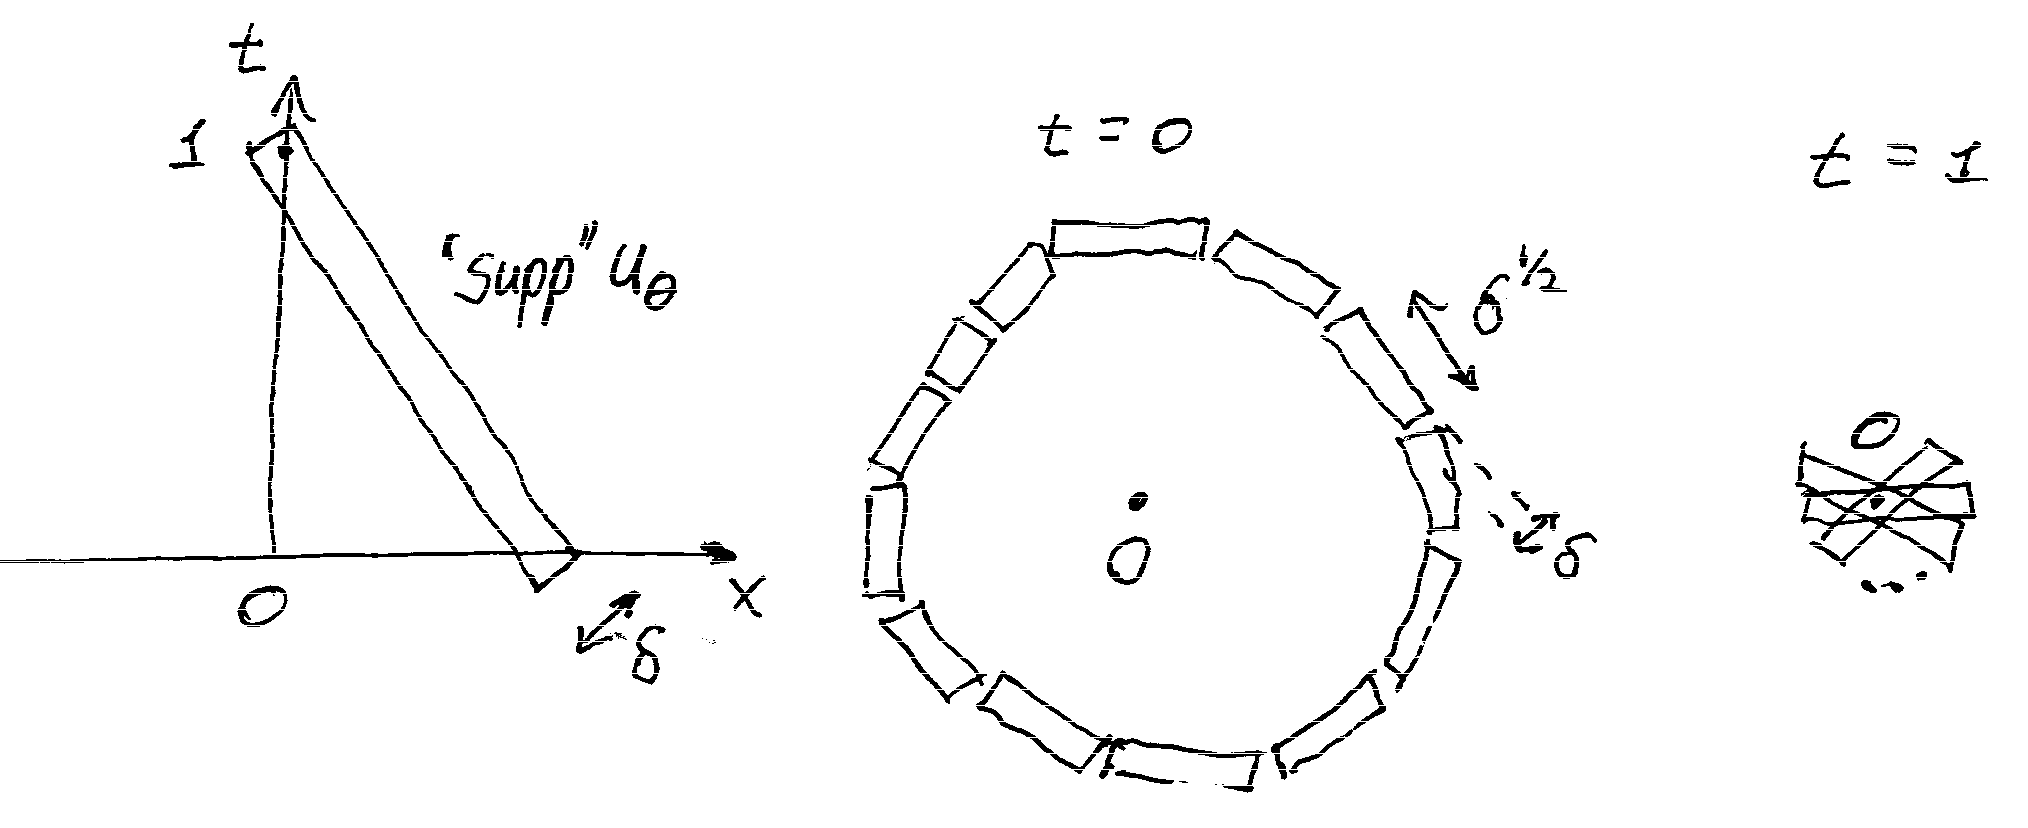
\includegraphics[width=\textwidth]{focusing-example.png}
\end{center}
\caption{Focusing example}
\end{figure}

Then, summing over a disjoint collection of $\theta$'s of cardinality $\approx \delta^{-(d-1)/2}$ we obtain
\[
\norm{\sum_{\theta}u_{\theta}(\cdot,t)}_{L^{p}(\R^{d})} \gtrsim \delta^{-(d-1)/2} \delta^{d/p}
\]
for $\abs{t-1} \lesssim \delta$.
On the other hand,
\[
\norm{\sum_{\theta}u_{\theta}(\cdot,0)}_{W^{\alpha,p}}
\sim
\delta^{1/p-\alpha}.
\]
Hence the fixed time estimate
\[
\norm{u(x,t)}_{L^{p}(\R^{d})}
\lesssim
\norm{f}_{W^{p,\alpha}}
\]
can only hold if $-(d-1)/2 + d/p \geq 1/p-\alpha$, or in other words $\alpha \geq \frac{d-1}{2} - \frac{d-1}{p}$.
The same example shows that the local smoothing estimate \eqref{eq:loc-smoothing} can only hold for $\alpha \geq \frac{d-1}{2} - \frac{d}{p}$.
Since by Theorem~\ref{thm:loc-smoothing:BD} the local smoothing estimate \eqref{eq:loc-smoothing} does hold in this range for sufficiently large $p$, it is better than what can be obtained from estimates for fixed times.
However, despite the name ``local smoothing'', the solution can still be less smooth than the initial data.
It seems that the name ``local smoothing'' comes from the Schr\"odinger equation, for which it is indeed the case that, on average over time, the solution is smoother than the initial data, see references in \cite{MR2456277}.

For a single $\theta$ the norm $\norm{u_{\theta}(\cdot,t)}_{L^{p}(\R^{d})}$ is morally constant for $\abs{t} \lesssim 1$.
Hence the local smoothing estimate \eqref{eq:loc-smoothing} can only hold for $\alpha \geq 0$.
It is conjectured that these two examples are essentially the worst.
\begin{conjecture}[{\cite{MR1098614}}]
\label{conj:loc-smoothing}
For $d\geq 2$ the estimate \eqref{eq:loc-smoothing} holds for $\alpha > \max(\frac{d-1}{2} - \frac{d}{p}, 0)$.
\end{conjecture}
Conjecture~\ref{conj:loc-smoothing} is not known in any dimension.
For $d\geq 3$ the best partial result is Theorem~\ref{thm:loc-smoothing:BD} (and an endpoint estimate \cite{MR2784663} for large $p$).
For $d=2$ two more results are known based on multilinear restriction \cite{MR2927399,arxiv:1607.08426}.
A possible route to Conjecture~\ref{conj:loc-smoothing} is via the chain of inequalities
\begin{equation}
\label{eq:path-to-local-smoothing}
\norm{u}_{L^{p}(\R^{d+1})}
\lessapprox
\norm{ \ell^{2}_{\theta} u_{\theta}}_{L^{p}(\R^{d+1})}
\lessapprox
\norm{ \ell^{2}_{\theta} f_{\theta}}_{L^{p}(\R^{d})}
\lessapprox
\norm{ f }_{L^{p}(\R^{d})}
\end{equation}
for the critical exponent $p = \frac{2 d}{d-1}$, where $\lesssim$ means that the implicit constant grows is $\lesssim_{\epsilon} \delta^{-\epsilon}$ for every $\epsilon>0$.
The first inequality in this chain would be stronger than the decoupling theorem (Theorem~\ref{thm:dec-cone}) since $L^{p} \ell^{2} \leq \ell^{2} L^{p}$.
The partial results concern this inequality.
The other two inequalities are in fact known for $d=2$, $p=4$.

Last inequality in \eqref{eq:path-to-local-smoothing} is proved in \cite{MR688026} (same argument is repeated in \cite{MR730074}) using a square function estimate from \cite{MR639467} and the estimate for the maximal function with $N$ directions in $\R^{d}$.

%%% Local Variables:
%%% mode: latex
%%% TeX-master: decoupling-notes
%%% End:
